% Options for packages loaded elsewhere
\PassOptionsToPackage{unicode}{hyperref}
\PassOptionsToPackage{hyphens}{url}
%
\documentclass[
]{article}
\usepackage{amsmath,amssymb}
\usepackage{lmodern}
\usepackage{ifxetex,ifluatex}
\ifnum 0\ifxetex 1\fi\ifluatex 1\fi=0 % if pdftex
  \usepackage[T1]{fontenc}
  \usepackage[utf8]{inputenc}
  \usepackage{textcomp} % provide euro and other symbols
\else % if luatex or xetex
  \usepackage{unicode-math}
  \defaultfontfeatures{Scale=MatchLowercase}
  \defaultfontfeatures[\rmfamily]{Ligatures=TeX,Scale=1}
  \setmainfont[]{Montserrat}
\fi
% Use upquote if available, for straight quotes in verbatim environments
\IfFileExists{upquote.sty}{\usepackage{upquote}}{}
\IfFileExists{microtype.sty}{% use microtype if available
  \usepackage[]{microtype}
  \UseMicrotypeSet[protrusion]{basicmath} % disable protrusion for tt fonts
}{}
\makeatletter
\@ifundefined{KOMAClassName}{% if non-KOMA class
  \IfFileExists{parskip.sty}{%
    \usepackage{parskip}
  }{% else
    \setlength{\parindent}{0pt}
    \setlength{\parskip}{6pt plus 2pt minus 1pt}}
}{% if KOMA class
  \KOMAoptions{parskip=half}}
\makeatother
\usepackage{xcolor}
\IfFileExists{xurl.sty}{\usepackage{xurl}}{} % add URL line breaks if available
\IfFileExists{bookmark.sty}{\usepackage{bookmark}}{\usepackage{hyperref}}
\hypersetup{
  pdftitle={PESKAS data report (testing version)},
  hidelinks,
  pdfcreator={LaTeX via pandoc}}
\urlstyle{same} % disable monospaced font for URLs
\usepackage[left=3cm,right=3cm,top=2cm,bottom=2cm]{geometry}
\usepackage{longtable,booktabs,array}
\usepackage{calc} % for calculating minipage widths
% Correct order of tables after \paragraph or \subparagraph
\usepackage{etoolbox}
\makeatletter
\patchcmd\longtable{\par}{\if@noskipsec\mbox{}\fi\par}{}{}
\makeatother
% Allow footnotes in longtable head/foot
\IfFileExists{footnotehyper.sty}{\usepackage{footnotehyper}}{\usepackage{footnote}}
\makesavenoteenv{longtable}
\usepackage{graphicx}
\makeatletter
\def\maxwidth{\ifdim\Gin@nat@width>\linewidth\linewidth\else\Gin@nat@width\fi}
\def\maxheight{\ifdim\Gin@nat@height>\textheight\textheight\else\Gin@nat@height\fi}
\makeatother
% Scale images if necessary, so that they will not overflow the page
% margins by default, and it is still possible to overwrite the defaults
% using explicit options in \includegraphics[width, height, ...]{}
\setkeys{Gin}{width=\maxwidth,height=\maxheight,keepaspectratio}
% Set default figure placement to htbp
\makeatletter
\def\fps@figure{htbp}
\makeatother
\setlength{\emergencystretch}{3em} % prevent overfull lines
\providecommand{\tightlist}{%
  \setlength{\itemsep}{0pt}\setlength{\parskip}{0pt}}
\setcounter{secnumdepth}{5}
\usepackage{float}
\floatplacement{figure}{H}
\usepackage{leading}
\leading{16pt}
\usepackage{caption}
\captionsetup[figure]{font=small}
\captionsetup[table]{font=small}
\definecolor{myblue}{RGB}{68,117,151}
\let\counterwithout\relax
\let\counterwithin\relax
\usepackage{chngcntr}
\counterwithin{figure}{section}
\ifluatex
  \usepackage{selnolig}  % disable illegal ligatures
\fi

\title{PESKAS data report (testing version)}
\author{}
\date{\vspace{-2.5em}}

\begin{document}
\maketitle

{
\setcounter{tocdepth}{2}
\tableofcontents
}
\begin{center}\rule{0.5\linewidth}{0.5pt}\end{center}

\hypertarget{aim}{%
\section{Aim}\label{aim}}

This report summarises relevant statistics and insights from the Peskas platform during the period Jul 2017 - Nov 2021. The report examines the main temporal trends in the national revenue related to small-scale fishing in Timor-Leste and provides quantitative and qualitative information on the catches.

\hypertarget{revenue}{%
\section{Revenue}\label{revenue}}

The landing value in USD is obtained from landing surveys at multiple sites around the country. Fishers are asked for the estimated price of their catch at the landing site regardless of whether the catch is deemed for sale or consumption. Prices may change throughout the year and across landing sites. We then obtain monthly estimates using a random-effect statistical model.
\newline

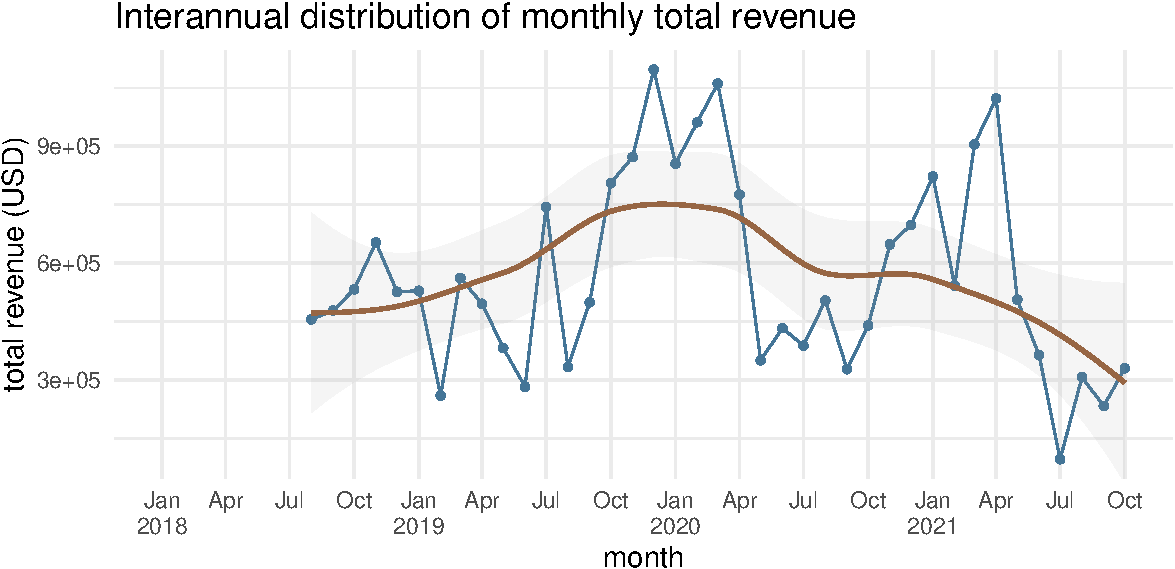
\includegraphics{data_report_files/figure-latex/unnamed-chunk-2-1.pdf}
\newline
\newline

\begin{figure}
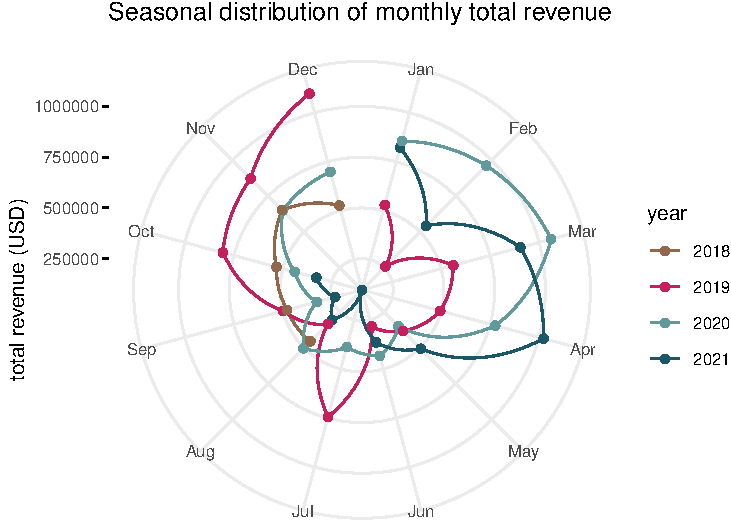
\includegraphics[width=0.9\linewidth,height=0.7\textheight]{data_report_files/figure-latex/unnamed-chunk-3-1} \caption{Monthly revenue shown for each year of Peskas' activity}\label{fig:unnamed-chunk-3}
\end{figure}
\pagebreak

\hypertarget{catches}{%
\section{Catches}\label{catches}}

Through the KoBo toolbox digital surveys, fishermen share several information related to each fishing trip. The fishermen were trained to provide homogeneous data both on the quality of the catch (the type of species caught) and on the quantity, indexed by the number of individuals and their length. In particular, the species caught are categorized in a list that includes the main species and groups caught in Timor-Leste (Table \ref{tab:catch-table}).
\newline



\begin{figure}
\includegraphics[width=1\linewidth,height=1\textheight]{data_report_files/figure-latex/overall-prop-1} \caption{Overall proportion of economic value and weight for each catch type.}\label{fig:overall-prop}
\end{figure}



\begin{figure}
\includegraphics[width=1\linewidth,height=1\textheight]{data_report_files/figure-latex/catch-value-1} \caption{Catches ranked by average value (USD). The darkest shade in each bar represent the 95\% confidence interval for average, other shades indicate the 5th and the 25th, and the 75th and 95th going from left to right respectively.}\label{fig:catch-value}
\end{figure}

\begin{figure}
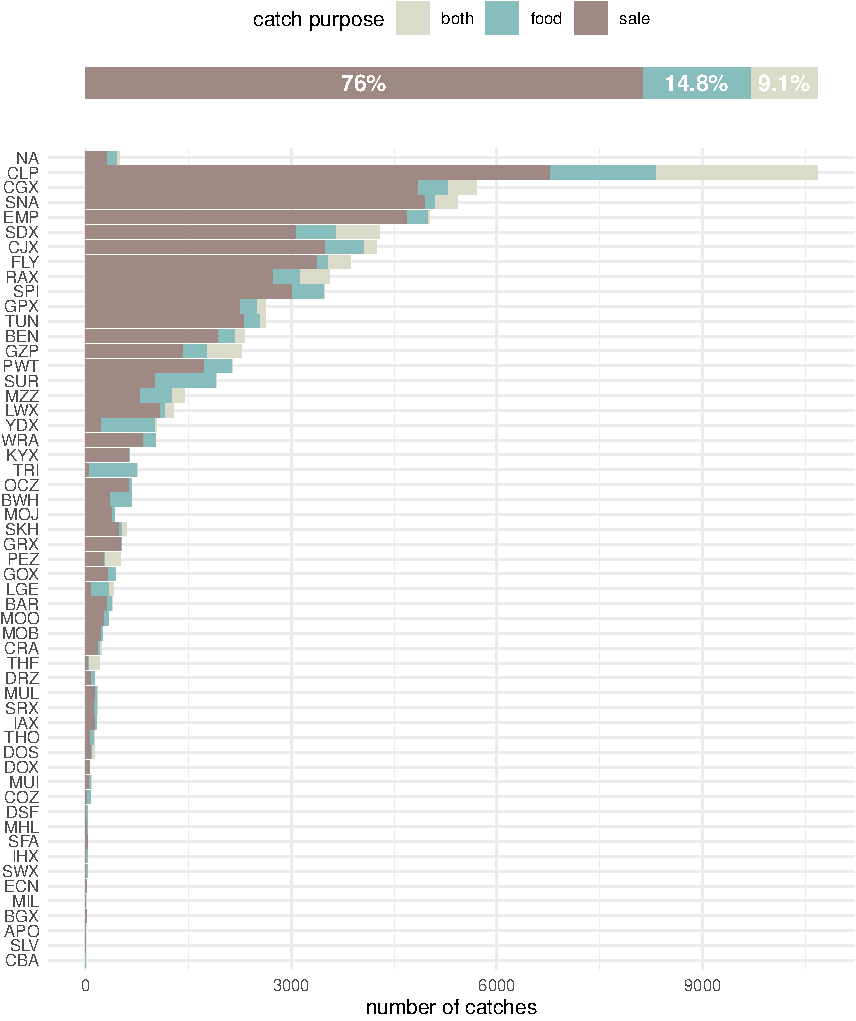
\includegraphics[width=1\linewidth,height=1\textheight]{data_report_files/figure-latex/unnamed-chunk-4-1} \caption{Total proportion of catches final usage (top) and usage proportion of each catch ranked by total number of catches (bottom)}\label{fig:unnamed-chunk-4}
\end{figure}

\begin{figure}
\centering
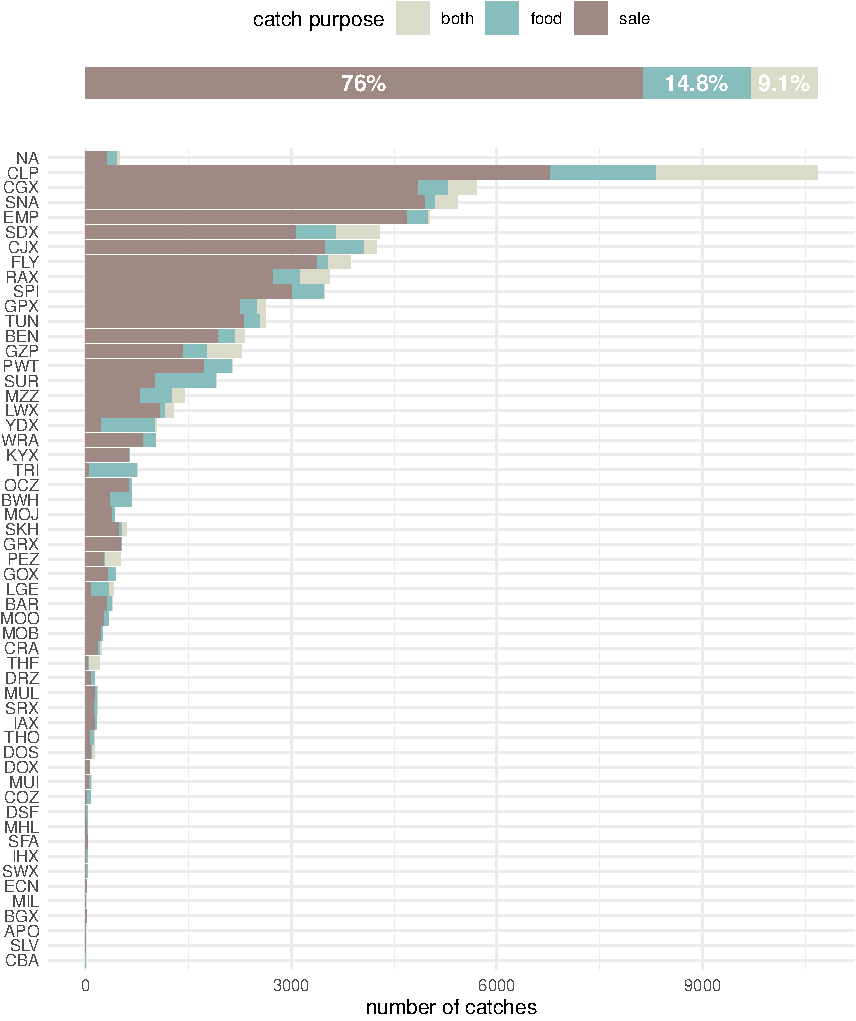
\includegraphics{data_report_files/figure-latex/unnamed-chunk-5-1.pdf}
\caption{\label{fig:unnamed-chunk-5}Interannual proportion catches final usage}
\end{figure}

\begin{figure}
\centering
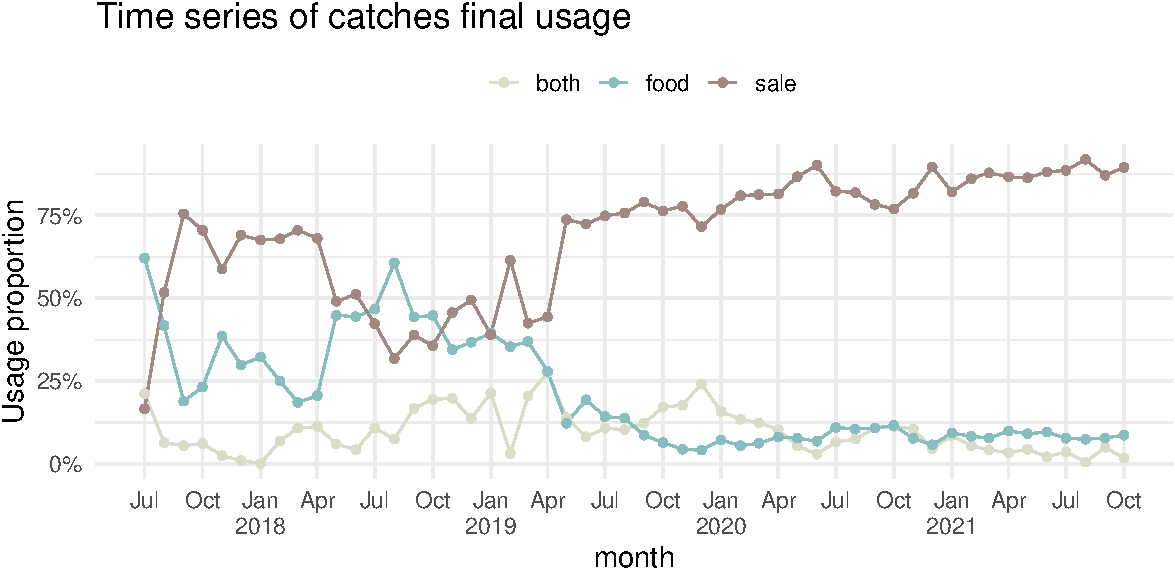
\includegraphics{data_report_files/figure-latex/unnamed-chunk-6-1.pdf}
\caption{\label{fig:unnamed-chunk-6}Time series of catches diversity on the monthly scale. Points represent average diversity while bars define the 0.95 confidence interval.}
\end{figure}

\begin{figure}
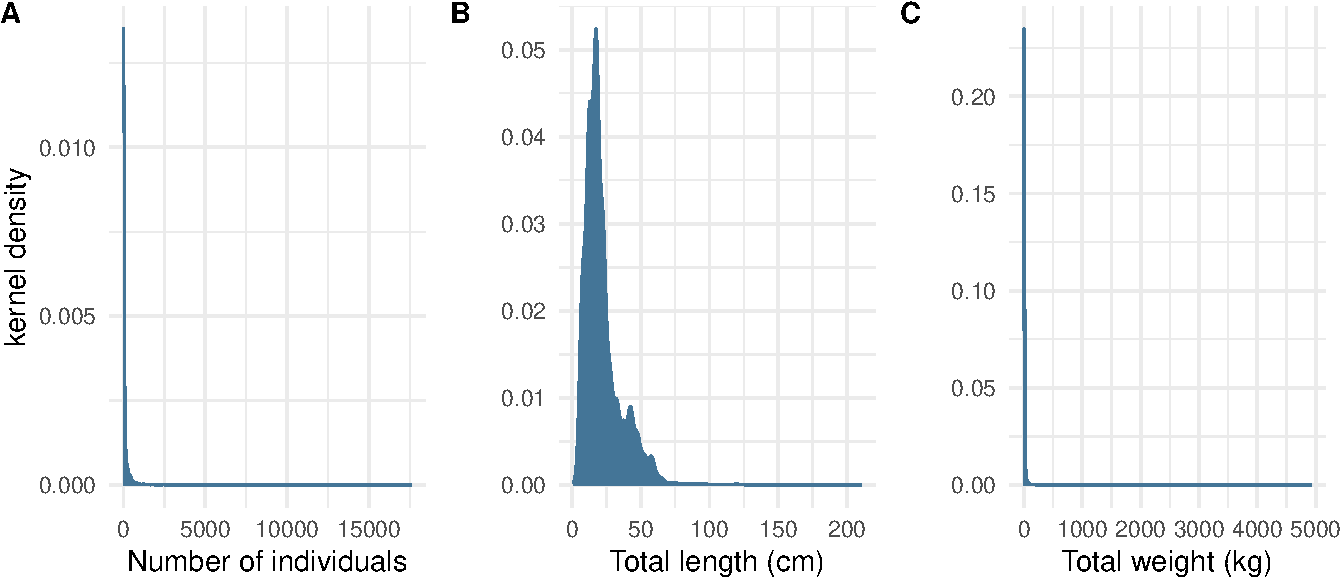
\includegraphics[width=1\linewidth,height=1\textheight]{data_report_files/figure-latex/unnamed-chunk-7-1} \caption{Main catches descriptors. Distribution of the number of individuals (A), their length (B)  and weigth (C) considering all the catches.}\label{fig:unnamed-chunk-7}
\end{figure}

\hypertarget{what-is-peskas}{%
\section{What is Peskas}\label{what-is-peskas}}

Peskas is the official fisheries national monitoring system of Timor-Leste and represents one of the most sophisticated data collection systems for small-scale fisheries in the world.

Peskas' platform collects real-time information directly from fishermen's activity via a system of digital surveys developed in \href{http://www.kobotoolbox.org/}{\(\color{myblue}{\text{KoBo toolbox}}\)}. In addition, Peskas uses the technology provided by \href{https://www.pelagicdata.com/}{\(\color{myblue}{\text{Pelagic Data System}}\)} to record vessel movements via solar-powered tracking devices (see Figure \ref{fig:flowchart}).

The data and the information collected is subjected to an elaborate processing and cleaning through an open-source code pipeline on \href{https://github.com/WorldFishCenter/peskas.timor.data.pipeline}{\(\color{myblue}{\text{GitHub}}\)}, and provide important data in the hands of fisheries officers, researchers and local stakeholders and enables them to better understand the contribution of fish and fisheries to local livelihoods and food security.

Information about the process and user-centred design of the Peskas pipeline and initial analytics, and its application in fisheries research \& management can be found in the following publications:

\begin{itemize}
\tightlist
\item
  \href{https://www.fao.org/documents/card/en/c/cb2030en}{\(\color{myblue}{\text{PeskAAS: A near real-time monitoring system for small-scale fisheries in Timor-Leste}}\)}. In A. Tilley \& M. B. Roscher (Eds.), Information and communication technologies for small-scale fisheries (ICT4SSF) - A handbook for fisheries stakeholders. In support of the implementation of the Voluntary Guidelines for Securing Sustainable Small-Scale Fisheries in the Context of Food Security and Poverty Eradication (pp.~11--18). FAO; WorldFish.
\item
  \href{https://journals.plos.org/plosone/article?id=10.1371/journal.pone.0234760}{\(\color{myblue}{\text{PeskAAS: A near-real-time, open-source monitoring and analytics system for small-scale fisheries}}\)}. PloS One, 15(11), e0234760.
\item
  \href{https://www.frontiersin.org/articles/10.3389/fmars.2019.00487/full}{\(\color{myblue}{\text{Nearshore Fish Aggregating Devices Show Positive Outcomes for Sustainable Fisheries Development in Timor-Leste}}\)}. Frontiers in Marine Science, 6, 487.
\end{itemize}



\begin{figure}
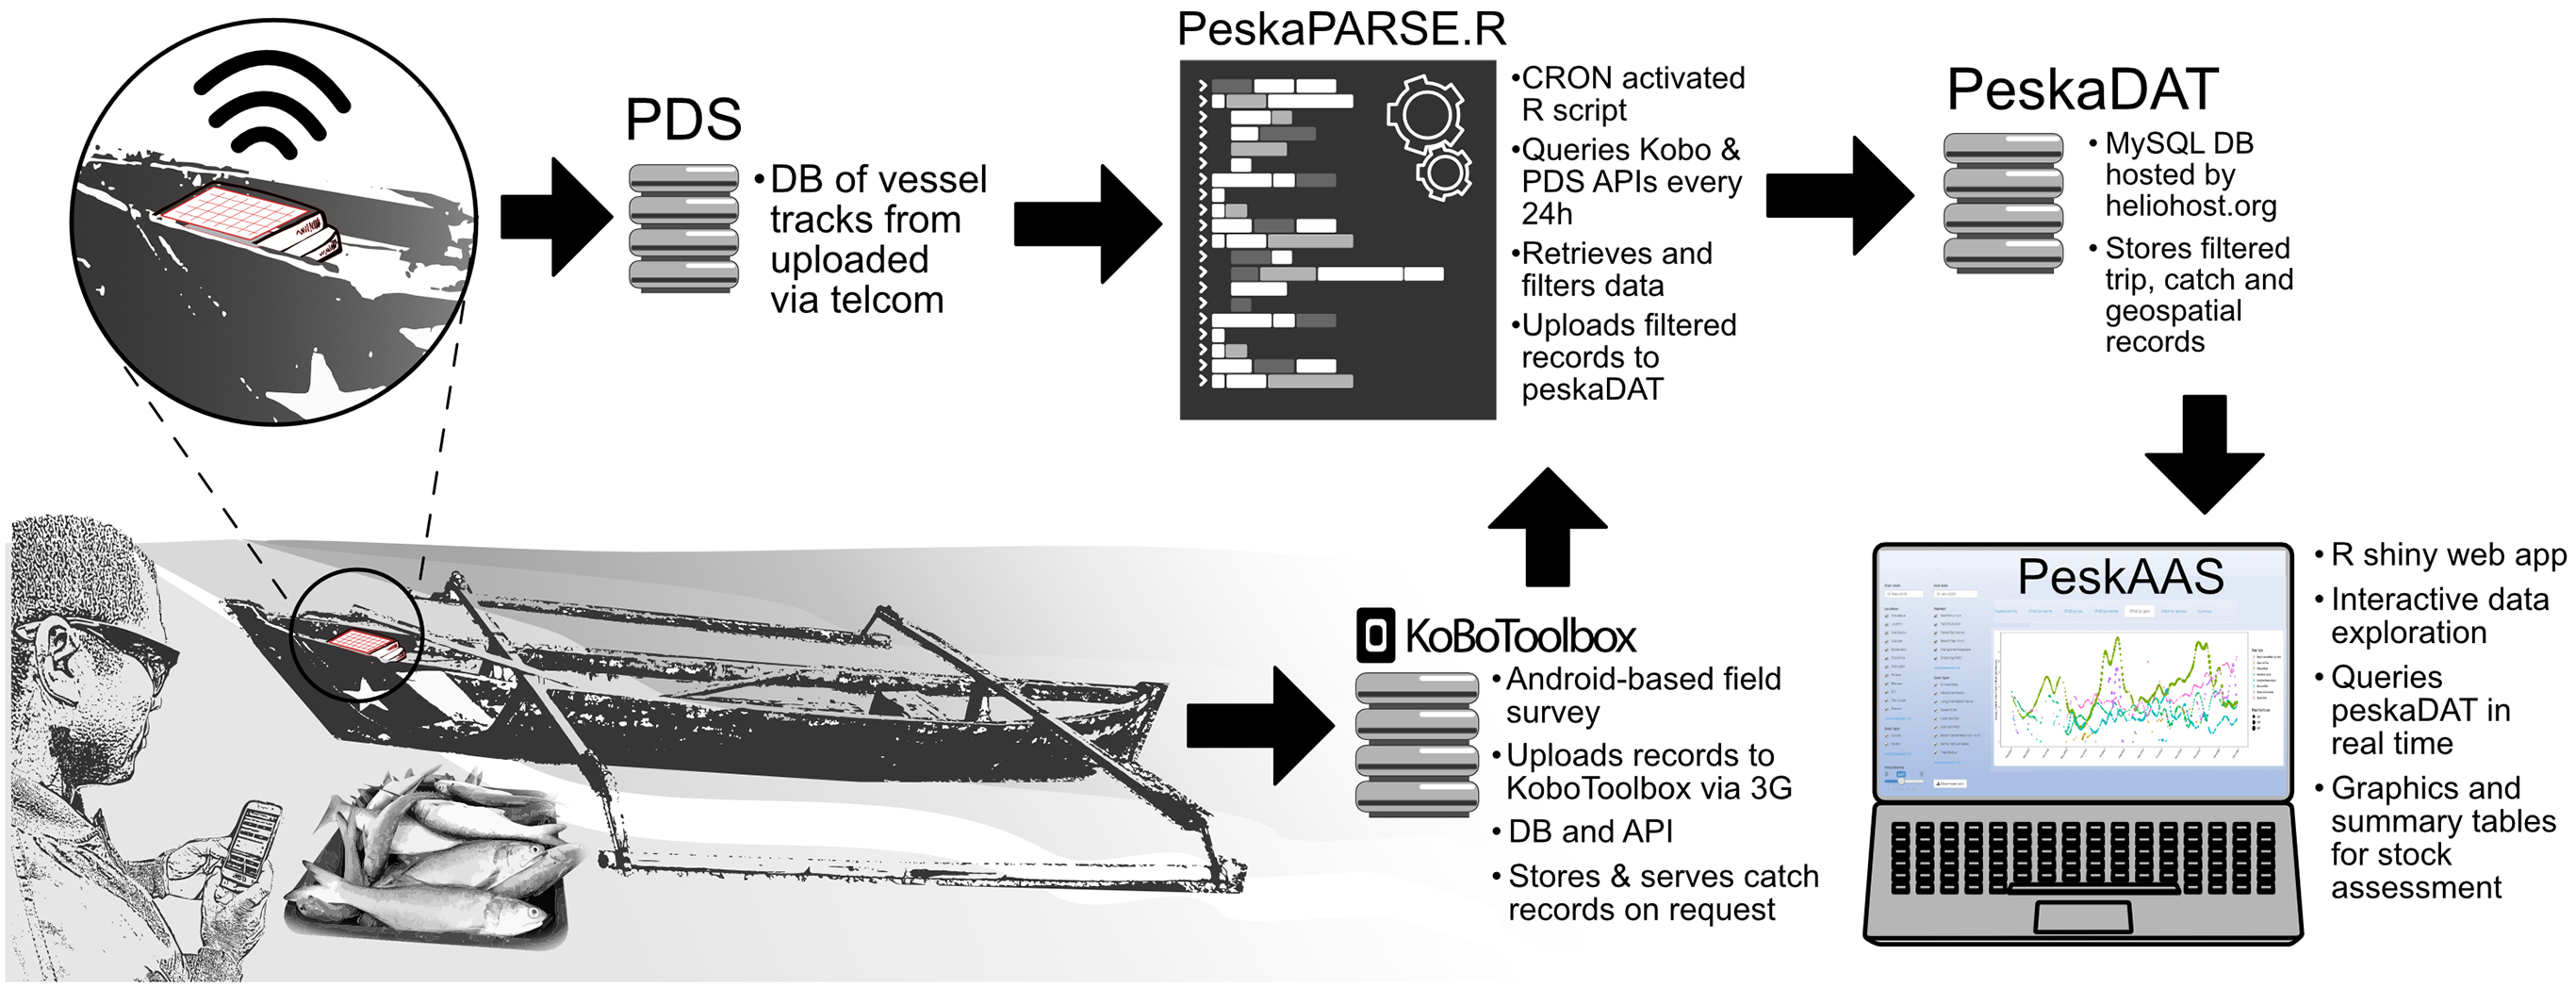
\includegraphics[width=37.96in]{inst/report_files/flowchart} \caption{A diagrammatic representation of the Peskas application. From \href{https://journals.plos.org/plosone/article?id=10.1371/journal.pone.0234760}{\(\color{myblue}{\text{PeskAAS: A near-real-time, open-source monitoring and analytics system for small-scale fisheries}}\)}}\label{fig:flowchart}
\end{figure}
\pagebreak

\begingroup\fontsize{7}{9}\selectfont

\begin{longtable}[t]{>{\centering\arraybackslash}p{6em}>{\centering\arraybackslash}p{18em}>{\centering\arraybackslash}p{18em}>{\centering\arraybackslash}p{18em}}
\caption{\label{tab:catch-table}ASFIS codes (FAO 3-Alpha Species Codes), scientific and common names of Peskas catches}\\
\toprule
\begingroup\fontsize{9}{11}\selectfont \textbf{n}\endgroup & \begingroup\fontsize{9}{11}\selectfont \textbf{ASFIS code}\endgroup & \begingroup\fontsize{9}{11}\selectfont \textbf{Taxonomic rank (family)}\endgroup & \begingroup\fontsize{9}{11}\selectfont \textbf{Common name}\endgroup\\
\midrule
\endfirsthead
\caption[]{\label{tab:catch-table}ASFIS codes (FAO 3-Alpha Species Codes), scientific and common names of Peskas catches \textit{(continued)}}\\
\toprule
\begingroup\fontsize{9}{11}\selectfont \textbf{n}\endgroup & \begingroup\fontsize{9}{11}\selectfont \textbf{ASFIS code}\endgroup & \begingroup\fontsize{9}{11}\selectfont \textbf{Taxonomic rank (family)}\endgroup & \begingroup\fontsize{9}{11}\selectfont \textbf{Common name}\endgroup\\
\midrule
\endhead

\endfoot
\bottomrule
\endlastfoot
\cellcolor{gray!6}{1} & \cellcolor{gray!6}{SKH} & \cellcolor{gray!6}{Carcharhinidae} & \cellcolor{gray!6}{Shark}\\
2 & PWT & Scaridae & Parrotfish\\
\cellcolor{gray!6}{3} & \cellcolor{gray!6}{GPX} & \cellcolor{gray!6}{Serranidae} & \cellcolor{gray!6}{Grouper}\\
4 & DRZ & Drepaneidae & Sicklefish\\
\cellcolor{gray!6}{5} & \cellcolor{gray!6}{THF} & \cellcolor{gray!6}{Polynemidae} & \cellcolor{gray!6}{Threadfin}\\
6 & PUX & Triacanthidae & Tripodfish\\
\cellcolor{gray!6}{7} & \cellcolor{gray!6}{GOX} & \cellcolor{gray!6}{Mullidae} & \cellcolor{gray!6}{Goatfish}\\
8 & BWH & Priacanthidae & Moontail bullseye\\
\cellcolor{gray!6}{9} & \cellcolor{gray!6}{BEN} & \cellcolor{gray!6}{Belonidae} & \cellcolor{gray!6}{Long tom}\\
10 & MUI & Muraenidae & Moray\\
\cellcolor{gray!6}{11} & \cellcolor{gray!6}{COZ} & \cellcolor{gray!6}{Cardiidae} & \cellcolor{gray!6}{Cockles}\\
12 & YDX & Holocentridae & Soldierfish\\
\cellcolor{gray!6}{13} & \cellcolor{gray!6}{OCZ} & \cellcolor{gray!6}{Octopodidae} & \cellcolor{gray!6}{Octopus}\\
14 & DOS & Chirocentridae & Wolf herring\\
\cellcolor{gray!6}{15} & \cellcolor{gray!6}{FLY} & \cellcolor{gray!6}{Exocoetidae} & \cellcolor{gray!6}{Flying fish}\\
16 & RAX & Scombridae & Short bodied mackerel\\
\cellcolor{gray!6}{17} & \cellcolor{gray!6}{MZZ} & \cellcolor{gray!6}{-} & \cellcolor{gray!6}{Other}\\
18 & THO & Terapontidae & Terapon\\
\cellcolor{gray!6}{19} & \cellcolor{gray!6}{DSF} & \cellcolor{gray!6}{Pomacentridae} & \cellcolor{gray!6}{Sergeant}\\
20 & SFA & Istiophoridae & Sailfish\\
\cellcolor{gray!6}{21} & \cellcolor{gray!6}{MOO} & \cellcolor{gray!6}{Menidae} & \cellcolor{gray!6}{Moonfish}\\
22 & CGX & Carangidae & Jacks/Trevally/Other Scad\\
\cellcolor{gray!6}{23} & \cellcolor{gray!6}{SUR} & \cellcolor{gray!6}{Acanthuridae} & \cellcolor{gray!6}{Unicornfish}\\
24 & APO & Apogonidae & Cardinalfish\\
\cellcolor{gray!6}{25} & \cellcolor{gray!6}{PEZ} & \cellcolor{gray!6}{-} & \cellcolor{gray!6}{Shrimp}\\
26 & IHX & Chaetodontidae & Butterflyfish\\
\cellcolor{gray!6}{27} & \cellcolor{gray!6}{MHL} & \cellcolor{gray!6}{Pempheridae} & \cellcolor{gray!6}{Blackspot sweeper}\\
28 & LGE & Leiognathidae & Ponyfish\\
\cellcolor{gray!6}{29} & \cellcolor{gray!6}{EMP} & \cellcolor{gray!6}{Lethrinidae} & \cellcolor{gray!6}{Emperor}\\
30 & MOB & Nemipteridae & Bream\\
\cellcolor{gray!6}{31} & \cellcolor{gray!6}{DOX} & \cellcolor{gray!6}{Coryphaenidae} & \cellcolor{gray!6}{Dolphinfish}\\
32 & SDX & Carangidae & Mackerel scad\\
\cellcolor{gray!6}{33} & \cellcolor{gray!6}{BAR} & \cellcolor{gray!6}{Sphyraenidae} & \cellcolor{gray!6}{Barracuda}\\
34 & - & - & No catch\\
\cellcolor{gray!6}{35} & \cellcolor{gray!6}{MIL} & \cellcolor{gray!6}{Chanidae} & \cellcolor{gray!6}{Milkfish}\\
36 & SRX & - & Stingrays\\
\cellcolor{gray!6}{37} & \cellcolor{gray!6}{IAX} & \cellcolor{gray!6}{Sepiidae} & \cellcolor{gray!6}{Cuttlefish}\\
38 & CRA & - & Crab\\
\cellcolor{gray!6}{39} & \cellcolor{gray!6}{CLP} & \cellcolor{gray!6}{Clupeidae} & \cellcolor{gray!6}{Sardines/pilchards}\\
40 & SWX & - & Seaweed\\
\cellcolor{gray!6}{41} & \cellcolor{gray!6}{CUX} & \cellcolor{gray!6}{-} & \cellcolor{gray!6}{Sea cucumber}\\
42 & BGX & Haemulidae & Javelin/Grunt\\
\cellcolor{gray!6}{43} & \cellcolor{gray!6}{MOJ} & \cellcolor{gray!6}{Gerreidae} & \cellcolor{gray!6}{Mojarra/Silverbelly}\\
44 & KYX & Kyphosidae & Chub\\
\cellcolor{gray!6}{45} & \cellcolor{gray!6}{LWX} & \cellcolor{gray!6}{Lutjanidae} & \cellcolor{gray!6}{Jobfish}\\
46 & IHX & Chaetodontidae & Bannerfish\\
\cellcolor{gray!6}{47} & \cellcolor{gray!6}{SPI} & \cellcolor{gray!6}{Siganidae} & \cellcolor{gray!6}{Spinefoot}\\
48 & TRI & Balistidae & Triggerfish\\
\cellcolor{gray!6}{49} & \cellcolor{gray!6}{SNA} & \cellcolor{gray!6}{Lutjanidae} & \cellcolor{gray!6}{Snapper/seaperch}\\
50 & CBA & Rachycentridae & Cobia\\
\cellcolor{gray!6}{51} & \cellcolor{gray!6}{SLV} & \cellcolor{gray!6}{-} & \cellcolor{gray!6}{Lobster}\\
52 & GZP & Hemiramphidae & Garfish\\
\cellcolor{gray!6}{53} & \cellcolor{gray!6}{TUN} & \cellcolor{gray!6}{Scombridae} & \cellcolor{gray!6}{Tuna/Bonito/Other Mackerel}\\
54 & MUL & Mugilidae & Mullet\\
\cellcolor{gray!6}{55} & \cellcolor{gray!6}{ECN} & \cellcolor{gray!6}{Echeneidae} & \cellcolor{gray!6}{Remora}\\
56 & GRX & Haemulidae & Sweetlips\\
\cellcolor{gray!6}{57} & \cellcolor{gray!6}{WRA} & \cellcolor{gray!6}{Labridae} & \cellcolor{gray!6}{Wrasse}\\
58 & CJX & Caesionidae & Fusilier\\*
\end{longtable}
\endgroup{}

\end{document}
